\documentclass[a4paper]{article} % Formato de Plantilla  que voy a utilizar

\usepackage[utf8]{inputenc} % Que me interprete todos los caracteres
\usepackage[spanish]{babel} % Se trabaja en español
\usepackage[margin=2cm, top=2cm, includefoot]{geometry}
\usepackage{graphicx} % Para la insercion de imagenes
\usepackage[table,xcdraw]{xcolor} % Para la deteción de colores
\usepackage[most]{tcolorbox} % Para la inserción de cuadros en la portada
\usepackage{fancyhdr} % Definir el estilo de la página
\usepackage{multirow} % Para centrar las palabras en las tablas
\usepackage[hidelinks]{hyperref} % Gestión de hipervinculos
\usepackage{listings} % Para la inserción de código en el documento
\usepackage{parskip} % Arreglo de la tabulación en el documento
\usepackage[figurename=Figura]{caption} % Cambiar el nombre del caption de las fotos
\usepackage{smartdiagram} % Para la inserción de diagramas
\usepackage{zed-csp} % Para la inserción de esquemas
\usepackage{pdfpages} % Para insertar PDF, en mi caso de Portada
\usepackage{tikz} % Para escribir encima del pdf
\usepackage{tabularray}

% Declaración de colores
\definecolor{blackPortada}{HTML}{000000} 
\definecolor{greenPortada}{HTML}{75d14f}
\definecolor{critico}{HTML}{b00505}
\definecolor{table1}{HTML}{2c83a8} % Color definido para la tabla1
\definecolor{lima}{HTML}{44f205} % Color para la tabla2 que son los Activos dentro del Alcance
\definecolor{gris}{HTML}{cdd1cf} % Color para la tabla2 que son los Activos dentro del Alcance

% Declaración de variables
\newcommand{\mylogo}{Images/maa.png} % My logo
\newcommand{\starDate}{15 de Febrero del 2024} % Fecha 

% Adicionales
\addto\captionsspanish{\renewcommand{\contentsname}{Índice}} % Cambio el formato del Índice
\setlength{\headheight}{40.2pt} % Espacio de la linea para insertar imagen en el encabezado
\pagestyle{fancy} % Estilo de la página
\fancyhf{} % Estilo de la página 
\fancyhead[L]{\href{https://0mariano.github.io}{\includegraphics[width=1.25cm]{\mylogo}}}
\fancyhead[R]{\begin{minipage}[b][1cm][c]{0.5\textwidth}\raggedleft\href{https://www.linkedin.com/in/mariano-alfonso-667a60226}{\textbf{MARIANO ALFONSO}}\end{minipage}} % Autor insertado en la derecha del encabezado
\renewcommand{\headrulewidth}{3pt} % Defino la anchura de la barra del encabezado
\renewcommand{\headrule}{\hbox to\headwidth{\color{blackPortada}\leaders\hrule height \headrulewidth\hfill}} % Definimos el color de la barra del encabezado
\renewcommand{\lstlistingname}{Código} % Cambio de nombre del caption de los códigos

\definecolor{codegreen}{rgb}{0,0.6,0} % Para insertar código
\definecolor{codegray}{rgb}{0.5,0.5,0.5}
\definecolor{codepurple}{rgb}{0.58,0,0.82}
\definecolor{backcolour}{rgb}{0.95,0.95,0.92}

\lstdefinestyle{mystyle}{
backgroundcolor=\color{backcolour},
commentstyle=\color{codegreen},
keywordstyle=\color{magenta},
numberstyle=\tiny\color{codegray},
stringstyle=\color{codepurple},
basicstyle=\ttfamily\footnotesize,
breakatwhitespace=false, 
frame=single,
breaklines=true,
captionpos=b,
keepspaces=true, 
numbers=left,
numbersep=5pt, 
showspaces=false, 
showstringspaces=false,
showtabs=false, 
 tabsize=2
}

\lstset{style=mystyle} % Termina la sintaxis para insertar código

% Comienzo del documento
\begin{document}
\cfoot{\thepage} % Numeros de páginas
% Creación de portada
\begin{titlepage}
\includepdf{Portada.pdf} % Inserto un pdf como portada
\end{titlepage}

% -----------------------------------------------------------------------------------------

% Comienzo del TOC (Table of Contens)
\clearpage
\tableofcontents
\clearpage
 
% -----------------------------------------------------------------------------------------

\section{Introducción}

En este \underline{Artículo}, nos adentraremos en dos pilares fundamentales del campo de la seguridad informática: la Triada CIA y el Cubo de McCumber. Estos conceptos son esenciales para comprender cómo proteger la información y los sistemas contra amenazas y ataques.\par 

El objetivo de este artículo no solo es proporcionar una comprensión básica de estos conceptos fundamentales, sino también fomentar la colaboración y el intercambio de conocimientos dentro de la comunidad de la \textbf{CiberSeguridad}, \textbf{Pentesting}, \textbf{Hacking Ético}.\par

\section{McCumber Cube}

En \textit{1991}, \textbf{John McCumber} lanzó un modelo de riesgo de ciberseguridad conocido como el cubo de McCumber.
Este modelo fue revolucionario por la forma en que describía los \textit{factores de riesgo de ciberseguridad} como un cubo
tridimensional. Cada una de las caras visibles del cubo tiene tres aspectos diferentes del riesgo en ciberseguridad que deben
gestionarse.

Los aspectos de cada dimensión son:

\begin{enumerate}
    \item Los principios fundamentales para proteger los sistemas de información.
    \item La protección de la información en cada uno de sus estados posibles.
    \item Las medidas de seguridad utilizadas para proteger los datos.
\end{enumerate}

\begin{figure}[h] % Con "h" indico que coloque la imagen abajo del texto
    \begin{center}
    \setlength{\fboxsep}{0.2em} % Ajustar la distancia del borde interno
    \fbox{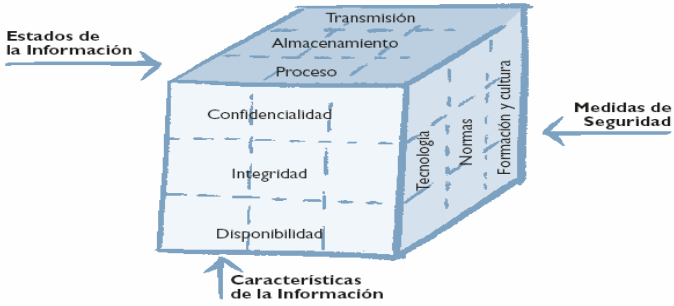
\includegraphics[width=1\textwidth]{Images/cube_McCumber.png}} % Utilizo \fbox para crear un borde alrededor de la imagen
    \end{center}
    \captionsetup{labelfont=bf} % Caption de la tabla en color negrita
    \caption{Cubo McCumber.}
\end{figure}

\vspace{3cm}

\section{Los principios fundamentales para proteger los sistemas de información}

    \subsection{Triada CIA}

    \vspace{0.2cm}

    Cuando nos referimos a la \textbf{Triada CIA}, estamos hablando de los conceptos de \textit{Confidencialidad}, \textit{Integridad} y \textit{Disponibilidad} (por sus siglas en inglés Confidentiality, Integrity, Availability). Es fundamental comprender el significado de estas palabras para desarrollar políticas y protocolos de seguridad informática que no solo protejan la información de posibles ataques de ciberdelincuentes, sino también al usuario al que pertenecen estos datos o que busca hacer uso de los mismos.

    \begin{figure}[h] % Con "h" indico que coloque la imagen abajo del texto
        \begin{center}
        \setlength{\fboxsep}{0.2em} % Ajustar la distancia del borde interno
        \fbox{
\includegraphics[width=0.5\textwidth]{Images/CIA-Triad.jpg}} % Utilizo \fbox para crear un borde alrededor de la imagen
        \end{center}
        \captionsetup{labelfont=bf} % Caption de la tabla en color negrita
        \caption{Triada CIA.}
    \end{figure}

        \subsubsection{Confidencialidad}
        
        Consiste en evitar que la información sensible sea revelada a personas no autorizadas, es decir, la información debe mantenerse en secreto y no debe divulgarse. De lo contrario, el pilar de confidencialidad de la Triada CIA se corrompería.

        \underline{\textit{\textcolor{blue}{Ejemplo}}}:
        
        Un claro ejemplo sería aquellas personas que trabajan en RR.HH. y manejan hojas de cálculo, cuentas bancarias, recibos de sueldo u otra información relacionada con el flujo de dinero. Por ello, no se otorgan permisos de acceso a la gran mayoría de otros empleados, y quizás incluso a ciertos ejecutivos. Si una organización tiene empleados que no pertenecen al área de RR.HH. y tienen acceso a cierta información a la que no deberían tener acceso, el pilar de confidencialidad no se cumple.

        Los métodos utilizados para garantizar la confidencialidad incluyen el \textbf{cifrado de datos}, la \textbf{autenticación} y el \textbf{control de acceso físico}.
        
        \vspace{2cm}

        \subsubsection{Integridad}

        Garantiza que la información sea confiable, consistente y precisa, protegiéndola contra modificaciones o alteraciones intencionales o accidentales, independientemente de cuánto tiempo haya pasado desde su creación. Si se protege la integridad de la información, se garantiza su confiabilidad y precisión.

        \underline{\textit{\textcolor{red}{Ejemplo}}}: 

        Una entidad bancaria debe garantizar que los datos de sus clientes no sean modificados o manipulados. Garantizar la integridad implica proteger los datos en uso, en tránsito (por ejemplo, al enviar un correo electrónico o al cargar o descargar un archivo) y al almacenarlos.
        
        Una forma de garantizar la integridad es utilizar \textbf{firmas digitales}.

        \subsubsection{Disponibilidad}

        Garantiza que la información esté disponible o accesible para personal autorizado siempre, cuando y donde sea necesario. Es decir, la capacidad de proporcionar acceso oportuno e ininterrumpido a los objetos depende tanto de la integridad como de la confidencialidad; sin ninguna de ellas, este pilar no se cumple.

        \underline{\textit{\textcolor{green}{Ejemplo}}}: 

        Supongamos que una empresa utiliza un sistema de gestión de inventario para llevar un registro preciso de su inventario y procesar pedidos de manera eficiente. Si este sistema experimenta una interrupción debido a un ataque, un error de hardware o un desastre natural, la disponibilidad se verá comprometida. Como resultado, los empleados no podrán acceder al sistema para realizar pedidos.

        La disponibilidad se puede proteger mediante el \textbf{mantenimiento} de los \textbf{sistemas operativos}, \textbf{actualizaciones de software} y \textbf{creando copias de seguridad}, así como la \textbf{implementación} o utilización de \textbf{servidores de alta disponibilidad}.
        
    Lograr que los tres elementos estén en equilibrio puede ser un desafío, pero idealmente, cuando se cumplen los tres pilares, el perfil de seguridad de la organización es más sólido y está mejor equipado para manejar incidentes de amenazas.

\section{La protección de la información en cada uno de sus estados posibles}  

    \subsection{Procesamiento}

    Se refiere a los datos que se utilizan para realizar una operación como la actualización de un registro de base de datos (datos en proceso)

    \subsection{Almacenamiento}

    Se refiere a los datos almacenados en la memoria o en un dispositivo de almacenamiento permanente, como un disco duro, una unidad de estado sólido o una unidad USB (datos en reposo)

    \subsection{Transmisión}

    Se refiere a los datos que viajan entre sistemas de información (datos en tránsito)

\vspace{2cm}

\section{Las medidas de seguridad utilizadas para proteger los datos} 

    \subsection{Awareness}

    Una organización debe implementar medidas de concientizacion mediante capacitaciones y educación sobre los empleados para que estén informados sobre las posibles amenazas a la seguridad y las acciones que pueden tomar para proteger los sistemas de información.

    \subsection{Tecnología}

    Se refiere a las soluciones basadas en software y hardware diseñadas para proteger los sistemas de información como los firewalls, que monitorean continuamente su red en busca de posibles incidentes maliciosos.

    \subsection{Políticas y el procedimientos}

    Se refiere a los controles administrativos que proporcionan una base para la forma en que una organización implementa el aseguramiento de la información, como los planes de respuesta a incidentes y las pautas de mejores prácticas.

\section{Apéndice I Links de Referencia}
       
    \subsection{Documentación}

    \begin{itemize}
        \item \href{https://skillsforall.com/course/introduction-to-cybersecurity?courseLang=en-US}{\textbf{\color{black}Cisco: Introducción a la Ciberseguridad}} \\
        \href{https://skillsforall.com/course/introduction-to-cybersecurity?courseLang=en-US}{\textbf{\color{blue}https://skillsforall.com/course/introduction-to-cybersecurity?courseLang=en-US}}
        \item \textbf{Wikipedia: McCumber cube} \\
        \href{https://en.wikipedia.org/wiki/McCumber_cube}{\textbf{\color{blue}https://en.wikipedia.org/wiki/McCumber\_cube}}
        \item \textbf{IBM: Conservación de la protección de datos
        en el mundo de la multicloud híbrida} \\
        \href{https://www.ibm.com/downloads/cas/OZ26LOBW}{\textbf{\color{blue}https://www.ibm.com/downloads/cas/OZ26LOBW}}
        \item \textbf{Fortinet: Tríada CIA: confidencialidad, integridad y disponibilidad} \\
        \href{https://www.fortinet.com/lat/resources/cyberglossary/cia-triad}{\textbf{\color{blue}https://www.fortinet.com/lat/resources/cyberglossary/cia-triad}}
    \end{itemize}   
    
\section{Contacto}

\begin{minipage}{0.05\textwidth}
  
\includegraphics[width=0.7\textwidth]{images/gmail.png} 
\end{minipage}
\begin{minipage}{.7\textwidth}
    \vspace{1mm} % Ajusta este valor según sea necesario para subir o bajar el bloque de texto
    \href{mailto:marianoalfonso80@protonmail.com}{\textbf{\color{black}E-mail}}: \href{mailto:marianoalfonso80@protonmail.com}{\textbf{\color{blue}marianoalfonso80@protonmail.com}}
\end{minipage} 

\begin{minipage}{0.05\textwidth}
    
\includegraphics[width=0.7\textwidth]{images/linkedin.png} 
\end{minipage}
\begin{minipage}{.7\textwidth}
    \vspace{1mm} % Ajusta este valor según sea necesario para subir o bajar el bloque de texto
    \href{https://www.linkedin.com/in/mariano-alfonso-667a60226}{\textbf{\color{black}LinkedIn}}: \href{https://www.linkedin.com/in/mariano-alfonso-667a60226}{\textbf{\color{blue}https://www.linkedin.com/in/mariano-alfonso-667a60226}}
\end{minipage} 

\begin{minipage}{0.05\textwidth}
    
\includegraphics[width=0.7\textwidth]{images/im_maa.png} 
\end{minipage}
\begin{minipage}{.7\textwidth}
    \vspace{1mm} % Ajusta este valor según sea necesario para subir o bajar el bloque de texto
    \href{https://0mariano.github.io}{\textbf{\color{black}Blog}}: \href{https://0mariano.github.io}{\textbf{\color{blue}https://0mariano.github.io}}
\end{minipage}

\begin{minipage}{0.05\textwidth}
    
\includegraphics[width=0.7\textwidth]{images/github.png} 
\end{minipage}
\begin{minipage}{.7\textwidth}
    \vspace{1mm} % Ajusta este valor según sea necesario para subir o bajar el bloque de texto
    \href{https://github.com/0mariano}{\textbf{\color{black}GitHub}}: \href{https://github.com/0mariano}{\textbf{\color{blue}https://github.com/0mariano}}
\end{minipage}

\end{document}